\documentclass[12pt]{article}
\usepackage{bigints}
\usepackage{graphicx}			% Use this package to include images
\usepackage{amsmath}	
\usepackage{amssymb}
\usepackage{amsfonts}
\usepackage{polynom}
% A library of many standard math expressions
\graphicspath{ {./Images/} }
\usepackage[margin=1in]{geometry}% Sets 1in margins. 
\newcommand{\qed}[0]{$\blacksquare$}
\usepackage{fancyhdr}			% Creates headers and footers
\usepackage{enumerate}          %These two package give custom labels to a list
\usepackage[shortlabels]{enumitem}


% Creates the header and footer. You can adjust the look and feel of these here.
\pagestyle{fancy}
\fancyhead[l]{Aditya Gupta}
\fancyhead[c]{Math 134 Homework \#9}
\fancyhead[r]{\today}
\fancyfoot[c]{\thepage}
\renewcommand{\headrulewidth}{0.2pt} %Creates a horizontal line underneath the header
\setlength{\headheight}{15pt} %Sets enough space for the header
\begin{document}


\begin{enumerate}
\item [Project 10.5]
\begin{enumerate}
    \item [1. ]
    \begin{enumerate} 
    
    Since there is no horizontal acceleration ($x''(t) = 0$), the horizontal velocity is constant:
    \[
    x'(t) = v_0 \cos \theta
    \]
    Integrating $x'(t)$ with respect to $t$, and considering the initial position $x(0) = x_0$, we get:
    \[
    x(t) = (v_0 \cos \theta) t + x_0
    \]
    The vertical acceleration is due to gravity only, so:
    \[
    y''(t) = -g
    \]
    Integrating once:
    \[
    y'(t) = -g t + C_1
    \]
    The constant $C_1$ is the initial vertical velocity, $v_0 \sin \theta$, so:
    \[
    y'(t) = -g t + v_0 \sin \theta
    \]
    Integrating again to find $y(t)$, and considering $y(0) = y_0$:
    \[
    y(t) = -\frac{1}{2} g t^2 + (v_0 \sin \theta) t + y_0
    \]
\end{enumerate}
    \item [2. ]
    From the equation for $x(t)$:
\[
x(t) = (v_0 \cos \theta) t + x_0,
\]
solve for $t$:
\[
t = \frac{x - x_0}{v_0 \cos \theta}.
\]

Substitute $t = \frac{x - x_0}{v_0 \cos \theta}$ into the equation for $y(t)$:
\[
y(t) = -\frac{1}{2} g t^2 + (v_0 \sin \theta) t + y_0.
\]
This gives:
\[
y = -\frac{1}{2} g \left(\frac{x - x_0}{v_0 \cos \theta}\right)^2 + (v_0 \sin \theta) \left(\frac{x - x_0}{v_0 \cos \theta}\right) + y_0.
\]

\[
y = -\frac{g}{2 (v_0^2 \cos^2 \theta)} (x - x_0)^2 + \frac{\sin \theta}{\cos \theta} (x - x_0) + y_0.
\]
Simplifying further:
\[
y = -\frac{g}{2 v_0^2 \cos^2 \theta} (x - x_0)^2 + \tan \theta (x - x_0) + y_0.
\]
Thus, the equation of the trajectory in rectangular coordinates has been shown to be:
\[
y = -\frac{g}{2 v_0^2 \cos^2 \theta} (x - x_0)^2 + \tan \theta (x - x_0) + y_0.
\]

\item [3. ] 

\textbf{(a) Parametric equations for the trajectory:}  
Using the parametric equations:
\[
x(t) = (v_0 \cos \theta) t, \quad y(t) = -\frac{1}{2} g t^2 + (v_0 \sin \theta) t.
\]
Here, $x_0 = 0$ and $y_0 = 0$ because the projectile is launched from the origin. The equations become:
\[
x(t) = (v_0 \cos \theta) t, \quad y(t) = -\frac{1}{2} g t^2 + (v_0 \sin \theta) t.
\]

\textbf{(b) Find the range of the projectile:}  
The range is the horizontal distance when the projectile hits the ground ($y = 0$). From the equation for $y(t)$:
\[
y(t) = -\frac{1}{2} g t^2 + (v_0 \sin \theta) t = 0.
\]
Factoring $t$:
\[
t \left( -\frac{1}{2} g t + v_0 \sin \theta \right) = 0.
\]
This gives two solutions:
\[
t = 0 \quad \text{(initial position)} \quad \text{and} \quad t = \frac{2 v_0 \sin \theta}{g}.
\]
The range is the $x$-coordinate when $t = \frac{2 v_0 \sin \theta}{g}$:
\[
x = (v_0 \cos \theta) t = v_0 \cos \theta \cdot \frac{2 v_0 \sin \theta}{g}.
\]
Using $\sin(2\theta) = 2 \sin \theta \cos \theta$, the range becomes(after replacing in the value of g):
\[
\text{Range} = \frac{v_0^2 \sin(2\theta)}{32}.
\]

\textbf{(c) Time of impact:}  
The time of impact is $t = \frac{2 v_0 \sin \theta}{g}$, as calculated in part (b).

\textbf{(d) Maximize the range:}  
The range is maximized when $\sin(2\theta) = 1$ since $\sin(2\theta) \leq 1$ for all $\theta$ which occurs at $2\theta = \frac{\pi}{2}$, or $\theta = \frac{\pi}{4}$. Thus, the maximum range occurs at angle of:
\[
\theta = \frac{\pi}{2}
\]

\textbf{(e) Determine $\theta$ for $x = b$:}  
To find $\theta$ such that the projectile lands at $x = b$, use the range equation:
\[
b = \frac{v_0^2 \sin(2\theta)}{32}.
\]
Rearranging for $\sin(2\theta)$:
\[
\sin(2\theta) = \frac{32b}{v_0^2}.
\]
Thus, the angle $\theta$ can be found as:
\[
\theta = \frac{1}{2} \arcsin\left(\frac{32b}{v_0^2}\right).
\]

\item [4. ]
\textbf{(a)}
Plotting the function into a graphing utility, we get the maximum range to be $r = 60892.4$ft and maximum height to be $h = 8789.06$ft

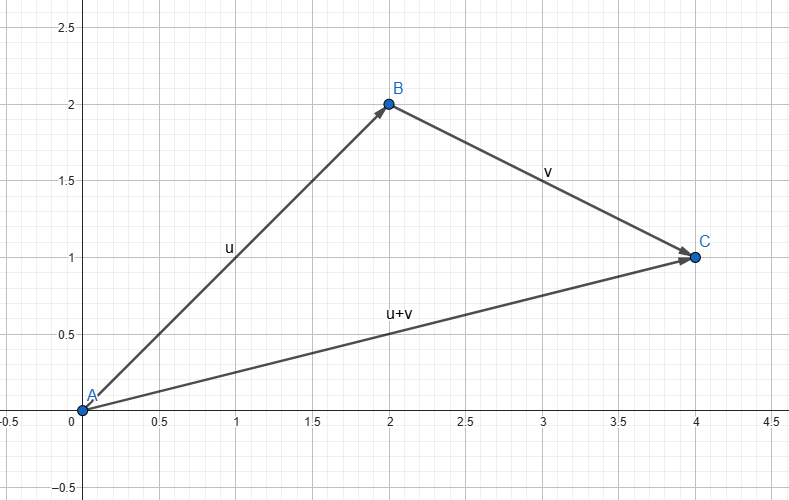
\includegraphics[width=0.5\linewidth]{Math 134//Images/image.png}

\textbf{(b)}

Using the formula for the range of the projectile:
\[
\text{Range} = \frac{v_0^2 \sin(2\theta)}{g},
\]
we calculate the range for several values of $\theta$ between $0^\circ$ and $90^\circ$.

\[
\text{Range} = \frac{1500^2 \sin(2\theta)}{32}.
\]
The calculations are shown in the following table:

\begin{center}
\begin{tabular}{|c|c|c|}
\hline
$\theta$ (degrees) & $\sin(2\theta)$ & Range (ft) \\ \hline
$10^\circ$ & $0.342$ & $24048.29$ \\ 
$20^\circ$ & $0.643$ & $45196.00$ \\ 
$30^\circ$ & $0.866$ & $60892.41$ \\ 
$40^\circ$ & $0.985$ & $69244.30$ \\ 
$45^\circ$ & $1.000$ & $70312.50$ \\ 
$50^\circ$ & $0.985$ & $69244.30$ \\ 
$60^\circ$ & $0.866$ & $60892.41$ \\ 
$70^\circ$ & $0.643$ & $45196.00$ \\ 
$80^\circ$ & $0.342$ & $24048.29$ \\ 
$90^\circ$ & $0.000$ & $0.00$ \\ \hline
\end{tabular}
\end{center}

From the table, it is evident that the range is maximized when $\theta = 45^\circ$, where the range is $70312.50 \, \text{ft}$. This confirms that the optimal angle for maximum range is $\theta = \frac{\pi}{4}$.




\end{enumerate}

\item [27. ]
To find the length of the curve defined by:
\[
x(\theta) = 3a \cos\theta + a \cos 3\theta, \quad y(\theta) = 3a \sin\theta - a \sin 3\theta,
\]
we use the formula for the length of a parametric curve:
\[
L = \int_0^{2\pi} \sqrt{\left(\frac{dx}{d\theta}\right)^2 + \left(\frac{dy}{d\theta}\right)^2} \, d\theta.
\]

First, compute the derivatives:
\[
\frac{dx}{d\theta} = -3a \sin\theta - 3a \sin 3\theta, \quad \frac{dy}{d\theta} = 3a \cos\theta - 3a \cos 3\theta.
\]

The sum of the squares of the derivatives is:
\[
\left(\frac{dx}{d\theta}\right)^2 + \left(\frac{dy}{d\theta}\right)^2 = (3a \sin\theta + 3a \sin 3\theta)^2 + (3a \cos\theta - 3a \cos 3\theta)^2.
\]

Expand each term:
\[
(3a \sin\theta + 3a \sin 3\theta)^2 = 9a^2 (\sin^2\theta + 2 \sin\theta \sin 3\theta + \sin^2 3\theta),
\]
\[
(3a \cos\theta - 3a \cos 3\theta)^2 = 9a^2 (\cos^2\theta - 2 \cos\theta \cos 3\theta + \cos^2 3\theta).
\]

Adding these:
\[
\left(\frac{dx}{d\theta}\right)^2 + \left(\frac{dy}{d\theta}\right)^2 = 9a^2 \left[(\sin^2\theta + \cos^2\theta) + (\sin^2 3\theta + \cos^2 3\theta) + 2 (\sin\theta \sin 3\theta - \cos\theta \cos 3\theta)\right].
\]

Using the Pythagorean identity \(\sin^2 x + \cos^2 x = 1\) and simplifying the cross terms:
\[
\sin\theta \sin 3\theta - \cos\theta \cos 3\theta = -\cos(3\theta - \theta) = -\cos 2\theta,
\]
we get:
\[
\left(\frac{dx}{d\theta}\right)^2 + \left(\frac{dy}{d\theta}\right)^2 = 9a^2 \left[2 - 2\cos 2\theta\right].
\]

Factoring out:
\[
\left(\frac{dx}{d\theta}\right)^2 + \left(\frac{dy}{d\theta}\right)^2 = 18a^2 (1 - \cos 2\theta).
\]

The square root becomes:
\[
\sqrt{\left(\frac{dx}{d\theta}\right)^2 + \left(\frac{dy}{d\theta}\right)^2} = \sqrt{18a^2 (1 - \cos 2\theta)} = 3a \sqrt{2(1 - \cos 2\theta)}.
\]

Using the trigonometric identity \(1 - \cos 2\theta = 2 \sin^2\theta\), we have:
\[
\sqrt{\left(\frac{dx}{d\theta}\right)^2 + \left(\frac{dy}{d\theta}\right)^2} = 3a \sqrt{4 \sin^2\theta} = 6a |\sin\theta|.
\]

 The modulus sign was added as $\sqrt{\sin^2(\theta)} \geq 0$ for all $\theta$.The length of the curve is:
\[
L = \int_0^{2\pi} 6a |\sin\theta| \, d\theta.
\]

Split the integral where \(\sin\theta\) changes sign:
\[
L = \int_0^\pi 6a \sin\theta \, d\theta - \int_\pi^{2\pi} 6a \sin\theta \, d\theta.
\]

Evaluate each integral:
\[
\int_0^\pi 6a \sin\theta \, d\theta = 6a [-\cos\theta]_0^\pi = 6a [-\cos\pi + \cos 0] = 6a [1 + 1] = 12a.
\]
\[
\int_\pi^{2\pi} 6a (-\sin\theta) \, d\theta = -6a \int_\pi^{2\pi} \sin\theta \, d\theta = -6a [-\cos\theta]_\pi^{2\pi} = -6a [-\cos(2\pi) + \cos(\pi)] = -6a [-1 + (-1)] = 12a.
\]

Adding the results:
\[
L = 12a + 12a = 24a.
\]

\item [43. ]
The arc length \(L\) of a curve \(y = f(x)\) from \(x = a\) to \(x = b\) is given by:
\[
L = \int_a^b \sqrt{1 + \left( \frac{dy}{dx} \right)^2} \, dx
\]

For \(y = \cosh(x)\), we have:
\[
\frac{dy}{dx} = \sinh(x)
\]
\[
\left( \frac{dy}{dx} \right)^2 = \sinh^2(x)
\]

Thus:
\[
L = \int_a^b \sqrt{1 + \sinh^2(x)} \, dx
\]

Using the identity \(1 + \sinh^2(x) = \cosh^2(x)\), we simplify:
\[
L = \int_a^b \cosh(x) \, dx
\]

The area under the curve \(y = \cosh(x)\) from \(x = a\) to \(x = b\) is:
\[
A = \int_a^b \cosh(x) \, dx
\]

Thus, we can see that the expressions for A and L are the same, proving the proposition.

\item [27.] The sphere has the equation \( x^2 + y^2 + z^2 = R^2 \), and its parametric representation is:
\( x(t) = R\cos t, y(t) = R\sin t \). 
For these, \( y'(t) = R\cos t \) and \( x'(t) = -R\sin t \). Substituting into the formula, we find:
\[
\sqrt{\left[x'(t)\right]^2 + \left[y'(t)\right]^2} = \sqrt{(-R\sin t)^2 + (R\cos t)^2} = R.
\]
Replacing in the value of the root expression, the surface area becomes:
\[
A = \int_c^d 2\pi y(t) R \, dt = \int_c^d 2\pi (R\sin t) R \, dt = 2\pi R^2 \int_c^d \sin t \, dt.
\]
\[
A = 2\pi R^2 \left[ -\cos t \right]_c^d = 2\pi R^2 \left( \cos c - \cos d \right).
\]
The planes intersect the sphere at \( z = h_1 \) and \( z = h_2 \), where \( z = R\cos t \), so \( \cos c = \frac{h_1}{R} \) and \( \cos d = \frac{h_2}{R} \). Substituting these, the surface area simplifies to:
\[
A = 2\pi R \left( h_1 - h_2 \right).
\]
Thus, the surface area of the band depends only on the distance \( |h_1 - h_2| \), not on the location of the planes.

\item [Project 10.8]

\begin{enumerate}
    \item [2. ]
\begin{enumerate}

The parametric equations for the cycloid are:
\[
x(\theta) = R(\theta - \sin\theta), \quad y(\theta) = R(1 - \cos\theta).
\]

The derivatives are:
\[
x'(\theta) = R(1 - \cos\theta), \quad y'(\theta) = R\sin\theta.
\]

At the end of each arch, \( \theta = 2n\pi \) (where \( n \) is an integer).

- Substituting \( \theta = 2n\pi \) into \( x'(\theta) \):
\[
x'(2n\pi) = R(1 - \cos(2n\pi)) = R(1 - 1) = 0.
\]

- Substituting \( \theta = 2n\pi \) into \( y'(\theta) \):
\[
y'(2n\pi) = R\sin(2n\pi) = R(0) = 0.
\]

Thus, \( x' \) and \( y' \) are both 0 at the end of each arch.

\item

\[
\text{Area} = \int_{0}^{2\pi} y(\theta) x'(\theta) \, d\theta.
\]

Using \( y(\theta) = R(1 - \cos\theta) \) and \( x'(\theta) = R(1 - \cos\theta) \):
\[
\text{Area} = \int_{0}^{2\pi} R(1 - \cos\theta) \cdot R(1 - \cos\theta) \, d\theta = R^2 \int_{0}^{2\pi} (1 - \cos\theta)^2 \, d\theta.
\]

Expanding \( (1 - \cos\theta)^2 \):
\[
(1 - \cos\theta)^2 = 1 - 2\cos\theta + \cos^2\theta.
\]

Substituting and splitting the integral:
\[
\text{Area} = R^2 \int_{0}^{2\pi} (1 - 2\cos\theta + \cos^2\theta) \, d\theta.
\]

The integrals of each term are:
1. \( \int_{0}^{2\pi} 1 \, d\theta = 2\pi \),
2. \( \int_{0}^{2\pi} \cos\theta \, d\theta = 0 \),
3. For \( \int_{0}^{2\pi} \cos^2\theta \, d\theta \), use the identity \( \cos^2\theta = \frac{1 + \cos(2\theta)}{2} \):
   \[
   \int_{0}^{2\pi} \cos^2\theta \, d\theta = \int_{0}^{2\pi} \frac{1}{2} \, d\theta + \int_{0}^{2\pi} \frac{\cos(2\theta)}{2} \, d\theta = \pi + 0 = \pi.
   \]

Substituting back:
\[
\text{Area} = R^2 (2\pi - 0 + \pi) = 3\pi R^2.
\]

The area of the rolling circle is \( \pi R^2 \). Thus, the area under an arch of the cycloid is three times the area of the rolling circle.

\item 

The length of an arch is given by:
\[
\text{Length} = \int_{0}^{2\pi} \sqrt{\left( x'(\theta) \right)^2 + \left( y'(\theta) \right)^2} \, d\theta.
\]

Using \( x'(\theta) = R(1 - \cos\theta) \) and \( y'(\theta) = R\sin\theta \):
\[
\text{Length} = \int_{0}^{2\pi} \sqrt{\left(R(1 - \cos\theta)\right)^2 + \left(R\sin\theta\right)^2} \, d\theta.
\]

Simplify the expression inside the square root:
\[
\left(R(1 - \cos\theta)\right)^2 + \left(R\sin\theta\right)^2 = R^2(1 - \cos\theta)^2 + R^2\sin^2\theta.
\]

Expanding \( (1 - \cos\theta)^2 \):
\[
(1 - \cos\theta)^2 = 1 - 2\cos\theta + \cos^2\theta.
\]

Substituting:
\[
R^2(1 - \cos\theta)^2 + R^2\sin^2\theta = R^2(1 - 2\cos\theta + \cos^2\theta) + R^2\sin^2\theta.
\]

Using \( \cos^2\theta + \sin^2\theta = 1 \):
\[
R^2(1 - 2\cos\theta + \cos^2\theta + \sin^2\theta) = R^2(1 - 2\cos\theta + 1) = R^2(2 - 2\cos\theta).
\]

Factor out \( 2R^2 \):
\[
\sqrt{R^2(2 - 2\cos\theta)} = R\sqrt{2(1 - \cos\theta)}.
\]

Using the trigonometric identity \( 1 - \cos\theta = 2\sin^2(\theta/2) \):
\[
R\sqrt{2(1 - \cos\theta)} = R\sqrt{2 \cdot 2\sin^2(\theta/2)} = 2R|\sin(\theta/2)|.
\]

Thus:
\[
\text{Length} = \int_{0}^{2\pi} 2R|\sin(\theta/2)| \, d\theta.
\]

Since \( |\sin(\theta/2)| \) is positive over \( [0, 2\pi] \):
\[
\text{Length} = 2R \int_{0}^{2\pi} \sin(\theta/2) \, d\theta.
\]

Let \( u = \theta/2 \), so \( d\theta = 2 \, du \), and the limits become \( u = 0 \) to \( u = \pi \):
\[
\text{Length} = 2R \cdot 2 \int_{0}^{\pi} \sin(u) \, du = 4R \left[-\cos(u)\right]_{0}^{\pi}.
\]

Evaluating:
\[
\text{Length} = 4R \left[-\cos(\pi) + \cos(0)\right] = 4R \left[-(-1) + 1\right] = 4R(2) = 8R.
\]

Thus, the length of an arch of the cycloid is \( 8R \).


\end{enumerate}
\item [3. ]
\begin{enumerate}
\item The centroid \((\bar{x}, \bar{y})\) of the region under the first arch is given by:
\[
\bar{x} = \frac{\int_{0}^{2\pi R} x \, y \, dx}{\int_{0}^{2\pi R} y \, dx}, \quad
\bar{y} = \frac{\int_{0}^{2\pi R} y^2 \, dx}{2\int_{0}^{2\pi R} y \, dx}.
\]

\( \bar{x} \): \( x \)-coordinate of the centroid
By symmetry of the cycloid about the vertical axis at \( x = \pi R \), the \( x \)-coordinate of the centroid is:
\[
\bar{x} = \pi R.
\]

\( \bar{y} \): \( y \)-coordinate of the centroid
The formula for \( \bar{y} \) is:
\[
\bar{y} = \frac{\int_{0}^{2\pi R} y^2 \, dx}{2\int_{0}^{2\pi R} y \, dx}.
\]

Step 1: Express \( dx \) in terms of \( d\theta \)
From the parametric equations:
\[
dx = x'(\theta) \, d\theta = R(1 - \cos\theta) \, d\theta.
\]

The bounds in terms of \( \theta \) are \( 0 \) to \( 2\pi \).

Step 2: Rewrite the numerator \( \int y^2 \, dx \)
Substitute \( y(\theta) = R(1 - \cos\theta) \):
\[
\int_{0}^{2\pi R} y^2 \, dx = \int_{0}^{2\pi} \big(R(1 - \cos\theta)\big)^2 R(1 - \cos\theta) \, d\theta.
\]

Simplify:
\[
\int_{0}^{2\pi R} y^2 \, dx = R^3 \int_{0}^{2\pi} (1 - \cos\theta)^3 \, d\theta.
\]

Expand \( (1 - \cos\theta)^3 \):
\[
(1 - \cos\theta)^3 = 1 - 3\cos\theta + 3\cos^2\theta - \cos^3\theta.
\]

Split the integral:
\[
\int_{0}^{2\pi} (1 - \cos\theta)^3 \, d\theta = \int_{0}^{2\pi} 1 \, d\theta - 3\int_{0}^{2\pi} \cos\theta \, d\theta + 3\int_{0}^{2\pi} \cos^2\theta \, d\theta - \int_{0}^{2\pi} \cos^3\theta \, d\theta.
\]

Evaluate each term:

1. \( \int_{0}^{2\pi} 1 \, d\theta = 2\pi \),

2. \( \int_{0}^{2\pi} \cos\theta \, d\theta = 0 \),

3. For \( \int_{0}^{2\pi} \cos^2\theta \, d\theta \), 
use \( \cos^2\theta = \frac{1 + \cos(2\theta)}{2} \):
   \[
   \int_{0}^{2\pi} \cos^2\theta \, d\theta = \int_{0}^{2\pi} \frac{1}{2} \, d\theta + \int_{0}^{2\pi} \frac{\cos(2\theta)}{2} \, d\theta = \pi + 0 = \pi.
   \]
   
4. \( \int_{0}^{2\pi} \cos^3\theta \, d\theta = 0 \) (by symmetry).

Thus:
\[
\int_{0}^{2\pi} (1 - \cos\theta)^3 \, d\theta = 2\pi - 0 + 3\pi - 0 = 5\pi.
\]

Substitute back:
\[
\int_{0}^{2\pi R} y^2 \, dx = R^3 \cdot 5\pi = 5\pi R^3.
\]

\[
\bar{y} = \frac{\int_{0}^{2\pi R} y^2 \, dx}{2\int_{0}^{2\pi R} y \, dx} = \frac{5\pi R^3}{2 \cdot 3\pi R^2}.
\]

Simplify:
\[
\bar{y} = \frac{5R}{6}.
\]

Thus, the centroid is located at:
\[
\left(\bar{x}, \bar{y}\right) = \left(\pi R, \frac{5R}{6}\right).
\]

\item 

Using Pappus's Centroid Theorem, the volume of revolution around x axis is given by:
\[
V_x = A \cdot (2\pi \cdot \bar{y}),
\]
where:
\[
A = 3\pi R^2, \quad \bar{y} = \frac{5R}{6}.
\]

Substitute:
\[
V_x = 3\pi R^2 \cdot 2\pi \cdot \frac{5R}{6}.
\]

Simplify:
\[
V_x = 3\pi R^2 \cdot \frac{10\pi R}{6} = 5\pi^2 R^3.
\]

Thus, the volume of revolution around the \(x\)-axis is:
\[
V_x = 5\pi^2 R^3.
\]


\item

\[
V_y = A \cdot (2\pi \cdot \bar{x}),
\]
where:
\[
A = 3\pi R^2, \quad \bar{x} = \pi R.
\]

Substitute:
\[
V_y = 3\pi R^2 \cdot 2\pi \cdot \pi R.
\]

Simplify:
\[
V_y = 3\pi R^2 \cdot 2\pi^2 R = 6\pi^3 R^3.
\]

Thus, the volume of revolution around the \(y\)-axis is:
\[
V_y = 6\pi^3 R^3.
\]

\end{enumerate}







\end{enumerate}
\end{enumerate}

\end{document}
